
\newpage
\subsection{Finite Automata Reduction (FAR)}\label{sec:FAR}








\usetikzlibrary {automata, positioning}
\begin{figure}[h]
    \centering
    \begin{subfigure}[t]{0.45\textwidth}
        \centering
        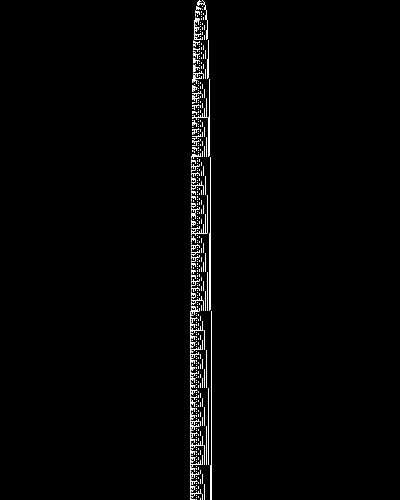
\includegraphics[width=0.85\textwidth]{figures/space-time-diagrams/counter_far.png}
        \caption*{}
    \end{subfigure}%
    \hfill
    \begin{subfigure}[t]{0.5\textwidth}
        \scalebox{0.8}{
            \begin{tikzpicture}[shorten >=1pt]
                \node[state,initial above] (0) at (-2, 2) {0};
                \node[state]           (1) at (-2, -2) {1};
                \node[state,accepting] (H) at (2, 4) {$\bot$};
                \node[state]           (0A) at (0, 2) {0A};
                \node[state,accepting] (0D) at (4, 2) {0D};
                \node[state]           (0B) at (2, 0) {0B};
                \node[state]           (0C) at (4, 0) {0C};
                \node[state]           (1C) at (2, -2.5) {1C};
                \node[state]           (1B) at (0, -4) {1B};
                \node[state]           (1A) at (4, -4) {1A};
                \node[state,accepting] (1D) at (5.5, -2) {1D};

                \path[->]  (0)  edge [loop right]       node {$0$} (0)
                edge                    node [right] {$1$} (1)
                (1)  edge [bend left=15]     node [above left] {$0|1$} (0)
                (0A) edge                    node [right] {$0$} (1B)
                edge                    node [above,rotate=60] {$1$} (H)
                (0C) edge                    node [above] {$0$} (0B)
                edge                    node [right] {$1$} (1A)
                (0D) edge                    node [above,rotate=300] {$0$} (H)
                edge                    node [above] {$1$} (0A)
                edge [bend left]        node [left] {$1$} (1A)
                (1A) edge                    node [above] {$1$} (1B)
                (1A) edge [bend right=15]    node [above,rotate=300] {$0|1$} (0B)
                (0B) edge [bend right=5]     node [above,rotate=300] {$0|1$} (1A)
                (1B) edge                    node [above right,rotate=60] {$0$} (0B)
                edge [loop left]        node {$0$} (1B)
                edge [bend left]        node [right] {$1$} (0A)
                (1C) edge                    node [above right,rotate=270] {$0|1$} (0B)
                (1D) edge [bend right=48]    node [below,rotate=300] {$0|1$} (H)
                (H)  edge [loop above]       node {$0|1$} (H)
                (0)  edge [dotted,bend left] node {\stateA} (0A)
                edge [dotted]           node [left] {\textcolor{colorB}{B}} (0B)
                edge [dotted]           node {\textcolor{colorC}{C}} (0C)
                edge [dotted,bend left] node [right] {\textcolor{colorD}{D}} (0D)
                (1)  edge [dotted]           node {\textcolor{colorB}{B}} (1B)
                edge [dotted]           node {\textcolor{colorA}{A}} (1A)
                edge [dotted]           node [left] {\textcolor{colorC}{C}} (1C)
                edge [dotted]           node [left] {\textcolor{colorD}{D}} (1D);
            \end{tikzpicture}
        }
        \label{fig:far_nfa}
    \end{subfigure}
    \caption[Short caption]{{\small Left: 20,000-step space-time diagram of 4-state machine \tm{1RB0LD_1LC1RA_0RB0LC_---1LA} -- we use a 4-state machine to have a small FAR Nondeterministic Finite Automaton (NFA). Right: NFA that satisfies the FAR conditions (Theorem~\ref{far-main-theorem}, with accepted steady state-set $\{\bot\}$) for this machine and hence is a certificate that the machine does not halt. This NFA accepts at least all eventually-halting configurations\footnotemark ~of the machine (configurations are represented as words, see Section~\ref{sec:FAR:theorem}); because it rejects the initial all-0 configuration (e.g. word-encoded as \texttt{A0}, or just \texttt{A}, not leading to an accept state), we know the machine does not halt.}}
    \label{fig:finite-automata-reduction}
\end{figure}

\footnotetext[\value{footnote}]{\label{fn:halting-caption}With finitely many \texttt{1}s, see Section~\ref{sec:FAR:theorem}.}
\vspace{-1em}
\subsubsection{Overview}

\newcommand{\M}{M}
\newcommand{\T}{^{T}}

Finite Automata Reduction (FAR) is a \textit{co-CTL} technique, \ie it is dual to the Closed Tape Language (CTL) framework given in Section~\ref{sec:deciders-overview}: for a given Turing machine, we are looking for a regular language that contains the set of the machine's eventually-halting configurations and, provided that the all-0 configuration is not in the regular language, we know that the machine does not halt.

The specificity of FAR is to restrict regular languages to a class of Nondeterministic Finite Automata (NFA) -- those satisfying Theorem~\ref{far-main-theorem} -- for which it is computationally simple to verify that they have the co-CTL properties: (i) reject the all-0 initial configuration, (ii) closed under Turing machine transitions, (iii) accept all eventually-halting configurations.

In \CoqBB, FAR is only used as a \textbf{verifier} meaning that specific Turing machines together with their FAR NFAs are directly hardcoded in the proof (in file \texttt{Verifier\_FAR\_Hardcoded\_Certificates.v}) and then verified using Theorem~\ref{far-main-theorem} -- see Section~\ref{sec:FAR:results} for results. FAR was originally developed as a fully-fledged decider -- \ie the verifier together with search algorithms for NFAs \cite{FAR,bbchallenge_part1}.

Here, we only present the verifier part of FAR (Theorem~\ref{far-main-theorem}) while we present the decider and its variations in \cite{bbchallenge_part1}. Figure~\ref{fig:finite-automata-reduction} (right) gives a FAR NFA (\ie satisfying\footnote{Using accepted steady state-set $\{\bot\}$, see Section~\ref{sec:FAR:theorem}.} Theorem~\ref{far-main-theorem}) for machine \tm{1RB0LD_1LC1RA_0RB0LC_---1LA}: the NFA accepts at least all the eventually-halting configurations\footref{fn:halting-caption} of the machine and rejects the initial all-0 configuration (\ie \texttt{A0} does not lead to an accept state), giving a certificate that the machine does not halt.

\subsubsection{FAR theorem}\label{sec:FAR:theorem}

In the following, we limit ourselves to Turing machines configurations with finite support, \ie configurations with finitely many \texttt{1}s (or, more generally, finitely many non-\texttt{0} symbols) and, when we write \textit{configuration}, we mean, \textit{configuration with finite support}.

A Turing machine configuration $c$ is represented as a finite word, called a \textit{word-representation} of $c$, by concatenating the tape content (from left to right, making sure to include all the \texttt{1}s) and adding the state (in our case, a letter from A to E) just before the position of the head, which is the same directional head notation used in Section~\ref{sec:RepWL}. For instance, two word-representations of the configuration $\texttt{0}^\infty \; \texttt{A> 0011} \; \texttt{0}^\infty$, are $\hat{c} = \texttt{A0011}$ and $\hat{c}' = \texttt{000A00110000}$. Similarly, the initial all-0 configuration can be encoded as \texttt{A0} or even just \texttt{A}. Word-representations of the same configuration will only differ in the number of leading and trailing \texttt{0}s that they have.


Then, a co-CTL regular language of word-represented configurations $\mathcal{L}$ for a Turing machine $\mathcal{M}$ satisfies:
\begin{align}
    u \in \mathcal{L}                               & \iff 0u \in \mathcal{L}           &  & \text{(leading zeros ignored)}
    \label{eq:lzignore}
    \\
    u \in \mathcal{L}                               & \iff u0 \in \mathcal{L}           &  & \text{(trailing zeros ignored)}
    \label{eq:tzignore}
    \\
    c\TMstep\bot                                    & \implies \hat{c} \in \mathcal{L}  &  & \text{(recognising halt, base case)} \nonumber \\
    (c_1\TMstep c_2)\land \hat{c}_2 \in \mathcal{L} & \implies\hat{c}_1 \in \mathcal{L} &  & \text{(recognising halt, induction)} \nonumber
\end{align}


With $c, c_1, c_2$ configurations of $\mathcal{M}$ (with finite support) and $\hat{c}, \hat{c}_1, \hat{c}_2$ any of their word-representations.


Given how word-representations are defined, the last two above conditions become:
\begin{align}
    \forall u,z\in\balphabet^*\!: \; ufrz \in \mathcal{L},\;                                                             & \text{if $\delta(f,r)$ is undefined (\ie halting)} \label{eq:h0}
    \\
    \forall u,z\in\balphabet^*,\,\forall b \in \balphabet\!: utbwz \in \mathcal{L} \implies ubfrz \in \mathcal{L},\;     & \text{if $\delta(f,r) = (w,\text{L},t)$} \label{eq:hnl}
    \\
    \forall u,z\in\balphabet^*,\,\forall b \in \balphabet\!: u w t z \in \mathcal{L} \implies u f r z \in \mathcal{L},\; & \text{if $\delta(f,r) = (w,\text{R},t)$} \label{eq:hnr}
\end{align}

With $f,t \in \{\stateA,\stateB,\stateC,\stateD,\stateE\}$ the ``from'' and ``to'' states in a transition, $r,w,b \in \balphabet$ the bit ``read'', the bit ``written'', and just a bit, and $\delta$ the transition table (see Section~\ref{sec:TMs}) of $\mathcal{M}$.


We now transform Conditions~\eqref{eq:lzignore}–\eqref{eq:hnr} into, sometimes stronger, conditions on the structure of NFAs -- using the usual linear-algebraic description of NFAs, which we first recall. Let $\mathbf{2}$ denote the Boolean semiring $\{0,1\}$ with operations $+$ and $\cdot$ respectively implemented by $\operatorname{OR}$ and $\operatorname{AND}$ \cite{CUNINGHAMEGREEN1991251}. Let $\M_{m,n}$ be the set of matrices with $m$ rows and $n$ columns over $\mathbf{2}$. We may define a Nondeterministic Finite Automaton (NFA) with $n$ states and alphabet $\mathcal{A}$ as a tuple $(q_0, \{T_\gamma\}_{\gamma \in \mathcal{A}}, a)$ where $q_0 \in \M_{1,n}$ and $a \in \M_{1,n}$ respectively represent the initial states and accepting states of the NFA. (i.e. if the $i^\text{th}$ state of the NFA is an initial state then the $i^\text{th}$ entry of $q_0$ is set to 1 and the rest are 0, and the $i^\text{th}$ entry of $a$ is set to 1 if and only if the $i^\text{th}$ state of the NFA is accepting), and where transitions are matrices $T_\gamma\in \M_{n,n}$ for each $\gamma\in\mathcal{A}$ (i.e. the entry $(i,j)$ of matrix $T_\gamma$ is set to 1 iff the NFA transitions from state $i$ to state $j$ when reading $\gamma$). Furthermore, for any word $u=\gamma_1\dots\gamma_\ell \in \mathcal{A}^*$, let $T_u = T_{\gamma_1} T_{\gamma_2} \dots T_{\gamma_\ell}$ be the state transformation resulting from reading word $u$ (note, $T_\epsilon = I$). A word $u=\gamma_1\dots\gamma_\ell \in \mathcal{A}^*$ is accepted by the NFA iff there exists a path from an initial state to an accepting state that is labelled by the symbols of $u$, which algebraically translates to $q_0 T_u a\T = 1$ with $a\T \in \M_{n,1}$ the transposition of $a$.

Using this algebraic framework\footnote{In the following, we limit ourselves to the binary tape alphabet $\balphabet$, but the results generalise transparently to arbitrary alphabets $\alphabet$.}, Conditions~\eqref{eq:lzignore}~and~\eqref{eq:tzignore} are implied by the following stronger conditions on transition matrix $T_0 \in \M_{n,n}$:
\begin{align}
    q_0 T_0 & = q_0
    \label{far-cond-leading-0}
    \\
    T_0 a\T & = a\T
    \label{far-cond-trailing-0}
\end{align}

Indeed, Condition~\eqref{far-cond-leading-0} transparently ignores leading zeros, Condition~\eqref{far-cond-trailing-0} means that for all accepting states of the NFA, reading a \szero is possible and leads to an accepting state since $T_0 a\T$ describes the set of NFA states that reach the set of accepting states $a$ after reading a \szero.

Then, Conditions~\eqref{eq:h0}--\eqref{eq:hnr} algebraically translate to:
{\small
\begin{align*}
    \forall u,z\in\balphabet^*\!: \; q_0 T_u T_f T_r T_z a\T = 1, \;                                                                             & \text{if $\delta(f,r)$ is undefined (\ie halting)}
    \\
    \forall u,z\in\balphabet^*,\,\forall b \in \balphabet\!: q_0 T_{u} T_t T_b T_w T_{z} a\T = 1 \implies q_0 T_{u} T_b T_f T_r T_{z} a\T = 1,\; & \text{if $\delta(f,r) = (w,\text{L},t)$}
    \\
    \forall u,z\in\balphabet^*,\,\forall b \in \balphabet\!: q_0 T_{u} T_w T_t T_{z} a\T = 1 \implies q_0 T_{u} T_f T_r T_{z} a\T = 1,\;         & \text{if $\delta(f,r) = (w,\text{R},t)$}
\end{align*}
}

These conditions are unwieldy. We seek stronger (thus still sufficient) conditions which are simpler:

\begin{itemize}

    \item For machine transitions going left or right, simply require $T_t T_b T_w\preceq T_b T_f T_r$ and $T_w T_t\preceq T_f T_r$, respectively, where $\preceq$ is the following relation on same-size matrices: $M\preceq M'$ if $M_{ij}\le M'_{ij}$ element-wise, that is, if the second matrix has at least the same 1-entries as the first matrix.

    \item To simplify the condition for halting machine transitions: define an \emph{accepted steady state-set} $s$ to be a row vector such that $sa\T = 1$, $s T_0\succeq s$, and $s T_1\succeq s$. Given such $s$, we have that: $\forall q\in\M_{1,n}\; q \succeq s\implies \forall z\in\balphabet^*\!: qT_{z}a\T = 1$. Assuming that such $s$ exists we can simply require: $\forall u\in\balphabet^*\!: q_0T_u T_f T_r \succeq s$ which is stronger than $\forall u,z\in\balphabet^*\!: \; q_0 T_u T_f T_r T_z a\T = 1$ where $\delta(f,r)$ is undefined.



\end{itemize}

Combining the above, we get FAR:



\begin{theorem}[\CoqBB: \texttt{Lemma dfa\_nfa\_verifier\_spec}\footnote{\CoqBB's lemma is slightly different, as it builds the NFA satisfying this theorem using a given ``precursor'' Deterministic Finite Automaton (DFA) -- as initially developed in \cite{FAR} -- see Section~\ref{sec:FAR:results}.}]
    \label{far-main-theorem}
    Machine $\mathcal{M}$, with transition table $\delta$ (see Section~\ref{sec:TMs}), does not halt from the initial all-0 configuration if there is a Nondeterministic Finite Automaton $(q_0, \{T_\gamma\}, a)$ and row vector $s$ satisfying the below:
    \begin{align}
        \label{far-cond-first}
        q_0 T_0                                    & = q_0
                                                   &                     & \text{(leading zeros ignored)}
        \tag{\ref{far-cond-leading-0}}
        \\
        T_0a\T                                     & = a\T
                                                   &                     & \text{(trailing zeros ignored)}
        \tag{\ref{far-cond-trailing-0}}
        \\
        sa\T                                       & = 1
                                                   &                     & \text{($s$ is accepted)}
        \label{far-cond-ass-accepted}
        \\
        sT_0,sT_1                                  & \succeq s
                                                   &                     & \text{($s$ is a steady state)}
        \label{far-cond-ass-steady}
        \\
        \forall u\in\balphabet^*\!: q_0T_u T_f T_r & \succeq s
                                                   &                     & \text{if $\delta(f,r)$ is undefined (\ie halting)}
        \label{far-cond-halt}
        \\
        \forall b\in\balphabet\!: T_b T_f T_r      & \succeq T_t T_b T_w
                                                   &                     & \text{if $\delta(f,r) = (w,\text{L},t)$}
        \label{far-cond-left}
        \\
        T_f T_r                                    & \succeq T_w T_t
                                                   &                     & \text{if $\delta(f,r) = (w,\text{R},t)$}
        \label{far-cond-last}
        \\
        q_0 T_A a\T                                & = 0
                                                   &                     & \text{(initial configuration rejected)}
        \label{far-cond-reject-start}
    \end{align}
\end{theorem}
\begin{proof}
    Conditions \eqref{far-cond-leading-0}--\eqref{far-cond-last} ensure that the NFA's language includes at least all eventually halting configurations of $\mathcal{M}$, see above. Condition~\eqref{far-cond-reject-start} ensures that the initial all-0 configuration of the machine is rejected, hence not eventually halting. Hence, if conditions \eqref{far-cond-leading-0}--\eqref{far-cond-reject-start} are satisfied, we can conclude that $\mathcal{M}$ does not halt from the initial all-0 configuration.
\end{proof}

\paragraph{Verifier.} Theorem~\ref{far-main-theorem} has the nice property of being easy to verify: given a Turing machine, an NFA and a vector $s$, the task of verifying that equations \eqref{far-cond-first}--\eqref{far-cond-reject-start} hold and thus that the machine does not halt, is computationally simple\footnote{Note that although equation~\eqref{far-cond-halt} has a $\forall u\in\balphabet^*$ quantification, the set of NFA states reachable after reading an arbitrary $u \in \balphabet^*$ is computable, and we just have to consider one instance of equation~\eqref{far-cond-halt} replacing $q_0 T_u$ per such state.}. For instance, it is easy to check that the NFA given in Figure~\ref{fig:finite-automata-reduction} satisfies Theorem~\ref{far-main-theorem}, using accepted steady state-set $\{\bot\}$, for machine \tm{1RB0LD_1LC1RA_0RB0LC_---1LA} and hence, the NFA provides a certificate that the machine does not halt.



\subsubsection{Implementations and results}\label{sec:FAR:results}

\CoqBB implements Theorem~\ref{far-main-theorem} in the special case where the FAR NFA is computed from a \textit{precursor} Deterministic Finite State Automaton, as described in \cite{bbchallenge_part1} (``direct FAR algorithm''). Certificates, consisting of such DFAs are hardcoded in the proof for 23 machines (in file \texttt{Verifier\_FAR\_Hardcoded\_Certificates.v}) and then verified using \texttt{dfa\_nfa\_verifier} (see file \texttt{Verifier\_FAR.v}).

These certificates were either found using extensive compute (\eg several weeks of searching DFAs essentially by brute force) or translated from other, undocumented, regular co-CTL methods (see Section~\ref{sec:deciders-overview}); indeed, in \cite{bbchallenge_part1} we show that FAR is an \textit{universal} regular co-CTL method: any regular co-CTL proof can be shoehorned into the framework of Theorem~\ref{far-main-theorem}.

\paragraph{Other implementations.} FAR has several other implementations: in Rust, C++ and Python~\cite{FAR,FAR_Tony,FAR_cosmo}.


























































































































































